\chapter{Numerical Root Finding}
Let's play a game!
\begin{problem}\label{prob:bisection_game}
    Find a partner in the room to play a two-person game.  Choose someone to go first and
    follow these steps to play.
    \begin{description}
        \item[Step \#1:] The first player secretly chooses a positive real number. For
            simplicity let's choose something less than 100.
        \item[Step \#2:] The first player chooses non-negative real numbers $a$ and $b$ so that the
            secret number is between $a$ and $b$.  
        \item[Step \#3:] The first player tells the second player ``{\it my number is between $a$
            and $b$}''.
        \item[Step \#4:] The second player makes a guess at the secret number.  We'll call
            that number $c$.
        \item[Step \#5:] The first player responds with one of the following three
            responses.
            \begin{itemize}
                \item If $c$ is within $0.01$ of the secret number then say\\ ``{\it you win!}''
                \item If the secret number is between $a$ and $c$ then say\\ ``{\it the secret
                number is between $a$ and $c$}.''
                \item If the secret number is between $c$ and $b$ then say\\ ``{\it the secret
                number is between $c$ and $b$}.''
            \end{itemize}
        \item[Step \#6:] Repeat steps 4 and 5 until the second player guesses the secret
            number to within $0.01$ or you have repeated more than 20 times. The second
            player wins if he/she guesses the number in 20 or fewer steps.
    \end{description}
\end{problem}

\begin{problem}
    Discuss with your partner what the optimal strategy for the second player is for the
    game in Problem \ref{prob:bisection_game}.
\end{problem}

\begin{problem}
    Now we want to write MATLAB code so you can play the game from Problem
    \ref{prob:bisection_game} against the computer.  The following incomplete code should
    get you started.  Fill in the missing pieces of the code and play the game several
    times to be sure that it works.  What strategy do you find yourself using to play the
    game? You can get a copy of the partial code
    \href{https://drive.google.com/file/d/1QFeb6ZGMppKtV-03_cbUzwaaKM8N39t2/view?usp=sharing}{HERE}.
\begin{lstlisting}
%% Secret Number Guesser Game
clear; clc; format compact;
secret = 100*rand(1,1); % random secret number between 0 and 100
tolerance = 0.01;
a = randi(floor(secret),1); % initial lower bound integer below the secret
b = randi( [ceil(secret),101] , 1); % initial upper bound integer above the secret
c = 1000; % dummy initial value for c
n = 1; % initialize the game counter
while abs( secret - c ) > tolerance
    fprintf('Guess #%g.\n',n)
    fprintf('The secret number is between %g and %g.\n',a,b)
    c = input('What is your guess for the secret number? ');
    if abs( secret - c ) < tolerance
        fprintf('  \n') % respond appropriately here
        ... % write more code here if necessary
    elseif secret < (c-tolerance)
        ... % write appropriate code here in this case
    elseif secret > (c+tolerance)
        ... % write appropriate code here in this case
    end
    if n>=20
        fprintf('   \n') % respond appropriately here
        break % this will break out of the loop
    end
    n=n+1; % increment the game counter
end
\end{lstlisting}
\end{problem}



\newpage
\section{Introduction to Root Finding}
In this chapter we want to solve algebraic equations using a computer.  Consider the equation
$\ell(x) = r(x)$ (where $\ell$ and $r$ stand for left and right respectively).  To solve
this equation we can first rewrite it by subtracting the right-hand side from the left to
get
\[ \ell(x) - r(x) = 0. \]
For example, if we want to solve $3\sin(x) + 9 = x^2 - \cos(x)$ then this is the same as
solving $(3\sin(x) + 9 ) - (x^2 - \cos(x)) = 0$.  Hence, we can define a function $f(x)$
as $f(x)=\ell(x)-r(x)$
and observe that \underline{every} algebraic equation can be written as: ``if $f(x) = 0$,
find $x$''.  We illustrate this idea in Figure \ref{fig:initial_root_example}.  On the
left-hand side of Figure \ref{fig:initial_root_example} we see the solutions to the
equation $3\sin(x) + 9 = x^2 - \cos(x)$, and on the right-hand side of Figure
\ref{fig:initial_root_example} we see the solutions to the equation $\left( 3\sin(x)+9
\right) - \left( x^2 - \cos(x) \right) = 0$.  From the plots it is apparent that the two
equations have the same solutions: $x_1 \approx -2.55$ and $x_2 \approx 2.88$.

\begin{figure}[ht!]
    \begin{center}
        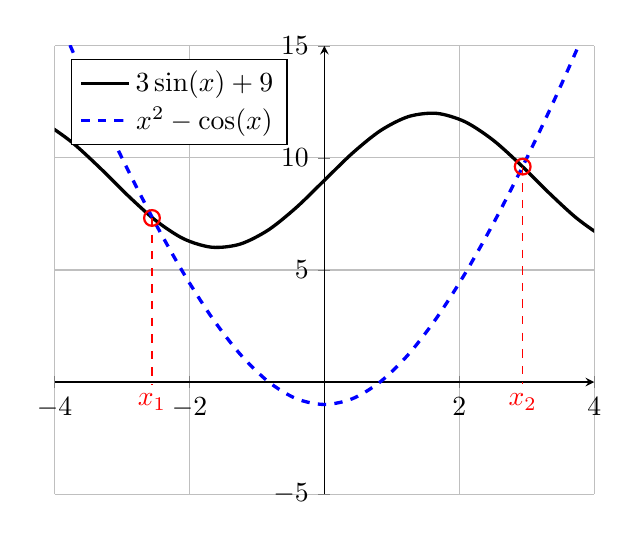
\begin{tikzpicture}
            \begin{axis}[axis lines=center, grid, xmin=-4, xmax=4, ymin=-5, ymax=15, legend
                pos=north west]
                \addplot[black, smooth, very thick] {3*sin(deg(x)) + 9};
                \addlegendentry{$3\sin(x) + 9$};
                \addplot[blue, smooth, dashed, very thick] {x^2 - cos(deg(x))};
                \addlegendentry{$x^2-\cos(x)$};
                \draw[thick, red] (axis cs:-2.556,7.32) circle(0.1cm);
                \draw[dashed, red] (axis cs:-2.556,7.32) -- (axis cs:-2.556,-0.1) node[anchor=north]{$x_1$};
                \draw[thick, red] (axis cs:2.94,9.61) circle(0.1cm);
                \draw[dashed, red] (axis cs:2.94,9.61) -- (axis cs:2.94,-0.1)
                node[anchor=north]{$x_2$};
            \end{axis}
        \end{tikzpicture}
        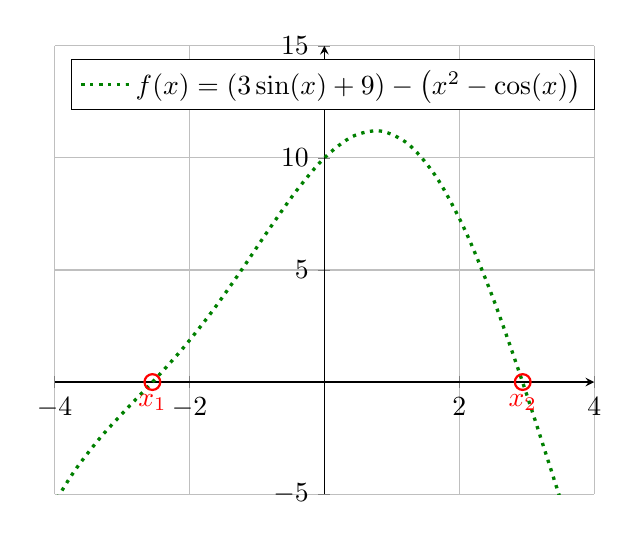
\begin{tikzpicture}
            \begin{axis}[axis lines=center, grid, xmin=-4, xmax=4, ymin=-5, ymax=15, legend
                pos=north west]
                \addplot[black!50!green, dotted, smooth, very thick] {3*sin(deg(x)) + 9 - x^2
                + cos(deg(x))};
                \addlegendentry{$f(x) = \left(3\sin(x) + 9\right) - \left( x^2-\cos(x)\right)$};
                \draw[thick, red] (axis cs:-2.55,0) circle(0.1cm);
                \draw[thick, red] (axis cs:-2.55,-0.1) node[anchor=north]{$x_1$};
                \draw[thick, red] (axis cs:2.94,0) circle(0.1cm);
                \draw[thick, red] (axis cs:2.94,-0.1) node[anchor=north]{$x_2$};
            \end{axis}
        \end{tikzpicture}
    \end{center}
    \caption{The left-hand plot shows two nonlinear functions, $\ell(x) = \sin(x) + 9$ and
        $r(x) = x^2 - \tan(x)$, with their intersection points marked. The right-hand plot
    shows the equivalent problem formed by solving $\ell(x) - r(x) = 0$.}
    \label{fig:initial_root_example}
\end{figure}

We now have one way to view every algebraic equation-solving problem.  As we'll see in
this chapter, if $f(x)$ has certain properties then different numerical techniques for
solving the equation will apply -- and some will be much faster and more accurate than
others. The following sections give several different techniques for solving algebraic
equations of the form $f(x) = 0$.

\newpage
\section{The Bisection Method}
We'll start the mathematical discussion with a theorem from Calculus.
\begin{thm}[The Intermediate Value Theorem (IVT)]
    If $f(x)$ is a continuous function on the closed interval $[a,b]$ and $y_*$ lies between
    $f(a)$ and $f(b)$, then there exists some point $x_* \in [a,b]$ such that $f(x_*) = y_*$.
    \label{thm:IVT}
\end{thm}


\begin{problem}
    Draw a picture of what the intermediate value theorem says graphically.
\end{problem}
\solution{
Draw a continuous function that crosses the line $y=y_*$ on the interval $[a,b]$.
}

\begin{problem}
    If $y_*=0$ the intermediate value theorem gives us important information about solving
    equations.  What does it tell us?
\end{problem}
\solution{
If $y_*=0$ and $f(x)$ is continuous then we know that there is a solution to the algebraic
equation $f(x) = 0$.
}

\begin{cor}
    If $f(x)$ is a continuous function on the closed interval $[a,b]$ and if $f(a)$ and $f(b)$ have opposite
    signs then from the Intermediate Value Theorem we know that there exists some point
    $x_* \in [a,b]$ such that \underline{\hspace{1in}}.
\end{cor}

Theorem \ref{thm:IVT} and its corollary are {\it existence theorems} in the sense that
they tell us that some point exists.  The annoying thing about mathematical existence
theorems is that they typically don't tell us {\it how} to find the point that is guaranteed to
exist -- annoying.
The following algorithm, known as the Bisection Method, uses the Intermediate
Value Theorem to systematically approximate the point $x_*$ to solve the algebraic
equation $f(x_*) =
0$.

\begin{problem}
    Discussion: What does the game from Problem \ref{prob:bisection_game} have in common
    with the Intermediate Value Theorem
    and its corollary?  Use your optimal strategy from the game along with
    the corollary to the IVT to propose a strategy to find roots of a continuous function.
    Write psuedo-code for your solution strategy.
\end{problem}

\begin{algorithm}[The Bisection Method]
    Assume that $f(x)$ is continuous on the closed interval $[a,b]$. To make approximations of
    the solutions to the equation $f(x) = 0$, do the following:
    \begin{enumerate}
        \item Check to see if $f(a)$ and $f(b)$ have opposite signs
            (why is this important?).\solution{In order for the IVT to apply you must have
            $0$ in between $f(a)$ and $f(b)$.}
        \item Compute the midpoint of the closed interval, $m=\frac{a+b}{2}$, and evaluate $f(m)$.
        \item Compare the signs of $f(a)$ vs $f(m)$ and $f(b)$ vs $f(m)$.  Replace one of
            the endpoints of the closed interval $[a,b]$ with $m=(a+b)/2$. (Which one do
            you replace and why?)
            \solution{Replace the endpoint where the function has the same sign as
                $f(m)$}
        \item Repeat steps 2 and 3 and stop when $f(m)$ is {\it close enough} to zero.
    \end{enumerate}
\end{algorithm}

\begin{problem}
    Draw a picture illustrating what the Bisection Method does to approximate solutions to
    the algebraic equation $f(x) = 0$.
\end{problem}


\begin{problem}
    We want to write a MATLAB function for the Bisection Method.  Instead of jumping
    straight into the code we should ALWAYS write pseudo-code first.  It is often helpful
    to write pseudo-code as comments in your MATLAB file.  Use the template below to
    complete your pseudo-code.
\begin{lstlisting}
function root = Bisection(f , a , b , tol)
% The input parameters are
% f is an anonymous function handle
% a is the lower guess
% b is the upper guess
% tol is an optional tolerance for the accuracy of the root

% if the user doesn't define a tolerance we need code to create a default

% check that there is a root between a and b
% if not we should return an error and break the code

% next calculate the midpoint m = (a+b)/2

% start a while loop
    % in the while loop we need an if statement
    % if ...
    % elseif ...
    % elseif ...

    % we should check that the while loop isn't running away

% end the while loop
% define the root
\end{lstlisting}
\end{problem}


\begin{problem}
    Now use the pseudo-code as structure to complete a MATLAB function for the Bisection
    Method.  Also write a test script that verifies that your function works properly. Be
    sure that it can take an anonymous function handle as an input along with an initial
    lower bound, an initial upper bound, and an optional error tolerance. The output
    should be only 1 single number: the root.\\
    \mcode{function root=Bisection(f , a , b , tol)}
\end{problem}

\begin{problem}
    Test your Bisection Method code on the following algebraic equations.
    \begin{enumerate}
        \item $x^2 - 2 = 0$ on $x \in [0,2]$ \solution{$\sqrt{2} \approx 1.414$}
        \item $\sin(x) + x^2 = 2\ln(x) + 5$ on $x \in [0,5]$ (be careful! make a plot
            first) \solution{$0.0860$ and $2.4953$ }
        \item $(5-x)e^{x}=5$ on $x \in [0,5]$\solution{$4.9651$}
    \end{enumerate}
\end{problem}


\begin{problem}
    Let $f(x)$ be a continuous function on the interval $[a,b]$ and assume that $f(a)
    \cdot f(b) <0$.  If we want to approximate the solution to the equation $f(x)=0$ to
    within $\delta$ how many iterations will the bisection method need? \\ Hint: If we
    want an approximation within $\delta$ then the width of the interval is $2\delta$.
\end{problem}
\solution{
    The width of the interval will always be half as large at each iteration.
    \begin{center}
        \begin{tabular}{|c|c|}
            \hline
            Iteration & Width of Interval \\ \hline \hline
            0 & $|a-b|$ \\
            1 & $\frac{|a-b|}{2}$ \\
            2 & $\frac{|a-b|}{2^2}$ \\
            \vdots & \vdots \\
            $k$ & $\frac{|a-b|}{2^k}$ \\
            \hline
        \end{tabular}
    \end{center}
    After $k$ steps the width of the interval is equal to $\frac{|a-b|}{2^k}$ so to reduce
    the interval to less than $2\delta$ we must have
    \[ \frac{|a-b|}{2^k} \le 2 \delta \implies \frac{|a-b|}{2\delta} \le 2^k \implies
        \frac{|a-b|}{\delta} \le 2^{k+1} \implies k \ge \log_2 \left(
        \frac{|a-b|}{\delta} \right) - 1 \]
}


\begin{problem}
    How many iterations of the bisection method are necessary to approximate $\sqrt{3}$ to
    within $10^{-3}$, $10^{-4}$, \dots, $10^{-15}$ using the initial interval
    $[a,b]=[0,2]$?
\end{problem}
\solution{
    \begin{center}
        \begin{tabular}{|c|c|}
            \hline
            Error & Num. Iterations \\ \hline \hline
            $10^{-3}$ & 10\\
            $10^{-4}$ & 14\\
            $10^{-5}$ & 17\\
            $10^{-6}$ & 20\\
            $10^{-7}$ & 24\\
            $10^{-8}$ & 27\\
            $10^{-9}$ & 30\\
            $10^{-10}$ & 34\\
            $10^{-11}$ & 37\\
            $10^{-12}$ & 40\\
            $10^{-13}$ & 44\\
            $10^{-14}$ & 47\\
            $10^{-15}$ & 50\\\hline
        \end{tabular}
    \end{center}
}



\newpage\section{The Regula Falsi Method}
The bisection method is one of many methods for performing root finding on a continuous
function.  The next algorithm takes a slightly different approach.

\begin{algorithm}[The Regula Falsi Method]
    Assume that $f(x)$ is continuous on the interval $[a,b]$. To make approximations of
    the solutions to the equation $f(x) = 0$, do the following:
    \begin{enumerate}
        \item Check to see if $f(a)$ and $f(b)$ have opposite signs so that the
            intermediate value theorem guarantees a root on the interval.
        \item Write the equation of the line connecting the points $(a,f(a))$ and
            $(b,f(b))$. Fill in the blanks in the point slope form.
            \[ y - \underline{\hspace{0.4in}} = \underline{\hspace{0.4in}} \cdot \left(
                x - \underline{\hspace{0.4in}} \right) \]
            \solution{
                \[ y - f(a) = \left( \frac{f(b) - f(a)}{b-a} \right) \left( x-a
                    \right) \]
            }
        \item Find the $x$ intercept of the linear function that you wrote in the previous
            step.  Call this point $x=c$.
            \[ c = \underline{\hspace{2in}} \]
            \solution{
                \[ 0 - f(a) = \left( \frac{f(b) - f(a)}{b-a} \right) \left( x-a
                    \right) \implies x = a+ \left( \frac{-f(a) (b-a)}{f(b)-f(a)} \right) \]
            }
        \item Just as we did with the bisection method, compare the signs of $f(a)$ vs
            $f(c)$ and $f(b)$ vs $f(c)$.  Replace one of the endpoints with $c$. Which one
            do you replace and why?
            \solution{Replace the endpoint where the function has the same sign as
                $f(c)$}
        \item Repeat steps 2 - 4, and stop when $f(c)$ is {\it close enough} to zero.
    \end{enumerate}
\end{algorithm}

\begin{problem}
    Draw a picture of what the Regula Falsi method does to approximate a root.
\end{problem}


\begin{problem}
    Give sketches of functions where the Regula Falsi method will perform faster than the
    Bisection method and visa versa.  Justify your thinking with several pictures and be
    prepared to defend your answers.
\end{problem}
\solution{
    The Regula Falsi method will perform very fast if the root is {\it close} to one of
    the chosen endpoints.  The bisection method will perform very vast if the root is {\it
    close} to the midoint of the two chosen endpoints.
}

\begin{problem}
    Create a new MATLAB function called \mcode{RegulaFalsi} and write comments giving pseudo-code
    for the Regula-Falsi method.
\end{problem}

\begin{problem}
   Use your pseudo-code to create a MATLAB function that implements the Regula Falsi method, and write a test script
   that verifies that your function works properly. Your function should accept an
    anonymous function handle as an input along with an initial lower bound, an initial
    upper bound, and an optional error tolerance. The output should be only 1 single number: the
    root.\\
    \mcode{function root=RegulaFalsi(f , a , b , tol)}
\end{problem}



\newpage\section{Newton's Method}
We now investigate a calculus-based method (originally proposed by Isaac Newton and later
modified by Joseph Raphson) for solving the algebraic equation $f(x)=0$. In very basic
terms, this method involves iteratively finding tangent lines to a differentiable curve
and locating where those tangent lines intersect the horizontal axis.
\begin{algorithm}[Newton's Method]
    The Newton-Raphson method for solving algebraic equations can be described as follows:
    \begin{enumerate}
        \item Check that $f$ is a twice differentiable function on a given domain and find
            a way to guarantee that $f$ has a root on that domain (this step happens by
            hand, not on the computer).
        \item Pick a starting point $x_0$ in the domain
        \item Write the equation of a tangent line to $f$ at $x_0$.  Fill in the blanks in
            the point-slope form.
            \[ y - \underline{\hspace{0.4in}} = \underline{\hspace{0.4in}} \cdot \left(
                x - \underline{\hspace{0.4in}} \right) \]
            \solution{
                \[ y - f(x_0) = f'(x_0) \left( x-x_0 \right) \]
            }
        \item Find the $x$ intercept of the equation of the tangent line and call this new
            point $x_1$.  
            \[ x_1 = \underline{\hspace{2in}} \]
            \solution{
                \[ x_1 = x_0 - \frac{f(x_0)}{f'(x_0)} \]
            }
        \item Now iterate the process by replacing the labels ``$x_1$'' and ``$x_0$'' in
            the previous step with $x_{n+1}$ and $x_{n}$ respectively.
            \[ x_{n+1} = \underline{\hspace{2in}} \]
            \solution{
                \[ x_{n+1} = x_{n} - \frac{f(x_n)}{f'(x_n)} \]
            }
        \item Iterate step 5 until $f(x_{n})$ is {\it close} to zero.
    \end{enumerate}
\end{algorithm}

\begin{problem}
    Draw a picture of what Newton's method does graphically.
\end{problem}

\begin{problem}\label{prob:newton_fail}
    There are several reasons why Newton's method could fail.  Work with your partners to
    come up with a list of all of the reasons.  Support each of your reasons with a
    sketch or an algebraic example.
\end{problem}
\solution{
    Newton's method will fail if
    \begin{itemize}
        \item the slope at the initial guess is zero (leading to no intersections of the
            tangent line with the $x$-axis), 
        \item the slope at any point in the interval is undefined,
        \item the initial guess is {\it too far away} from the intended root.
    \end{itemize}
}

\begin{problem}
    Create a new MATLAB function called \mcode{Newton} and write comments giving
    pseudo-code for Newton's method.  This version of Newton's method will accept the
    function and the first derivative so you don't need to set aside any code for
    calculating the derivative.
\end{problem}

\begin{problem}
    Write a MATLAB function for Newton's method.  Your function needs to accept an
    anonymous function handle, the derivative of $f(x)$ as an anonymous function handle, an initial
    guess, and an optional error
    tolerance. The only output should be the solution to the equation that you are
    solving.  Write a test script to verify that your Newton's method code indeed works.
    \\
    \mcode{function soln = Newton(f , df , x0 , tol)}
\end{problem}

\begin{problem}
    The previous problem required that you calculate the derivative ahead of time for
    Newton's method.  While this is relatively easy with a computer algebra system it
    might be easier just to have your function compute the derivative for you.  Write a
    new MATLAB function for Newton's method that accepts the function as an anonymous
    function handle, the initial point, and an optional error tolerance.  Your function
    must compute the derivative symbolically behind the scenes. \\
    \mcode{function soln = NewtonSymbolic(f, x0, tol)}
\end{problem}

\begin{problem}
    In Problem \ref{prob:newton_fail} you constructed several examples of where Newton's
    method will fail.  Modify your Newton's method code
    to catch these special cases and warns the user before the method fails.  Test your
    new code with several of the special cases showing that indeed you were able to catch
    them properly and give the user appropriate feedback.
\end{problem}


\begin{problem}\label{prob:newton_convergence}
    Newton's Method is known to have a {\it quadratic convergence rate}.  This means that 
    \[ \lim_{k \to \infty} \frac{|x_{k+1} - x_*|}{|x_k - x_*|^2} \]
    will be constant where $x_*$ is the root that we're hunting for.  This implies that
    if we plot the error in the new iterate on the $y$-axis and the error in the old
    iterate on the $x$ axis of a log-log plot then we will see a constant slope of 2.
    (stop and verify why this would be true).
    
    In this problem we're going to build a numerical experiment to verify that Newton's
    method indeed has quadratic convergence.  Modify your Newton's method code so that it
    outputs all of the iterations instead of just the final root.  Once you have the
    iterations compute the error between the approximations and the exact root. For
    simplicity let's solve the equation $x^2-2=0$.  Plot the sequence of error
    approximations with the iterate $e_k$ on the $x$-axis and the iterate $e_{k+1}$ on the
    $y$-axis of a log-log plot.  \\ Your plot command will look something like: \\
    \mcode{loglog(error(1:end-1),error(2:end),'b*')} \\where \mcode{error} is a vector
    containing all of the errors.  Quadratic convergence means that at every iteration the
    error should decrease by roughly 2 orders of magnitude.  How can you see this in your
    plot?
\end{problem}


\begin{problem}
    Repeat the previous problem with the bisection and regula falsi
    methods.  Plot the errors of all three methods on the same plot and discuss the rates
    of convergence for the three methods.
\end{problem}


\newpage\section{Quasi-Newton Methods}
Newton's method requires that you have a function and a derivative of that function.  The
conundrum here is that sometimes the derivative is cumbersome or impossible to obtain but
you still want to have the great quadratic convergence exhibited by Newton's method.

Recall that Newton's method is
\[ x_{n+1} = x_n - \frac{f(x_n)}{f'(x_n)}. \]
If we replace $f'(x_n)$ with an approximation of the derivative then we may have a method
that is {\it close} to Newton's method in terms of convergence rate but is less
troublesome to compute. Any method that replaces the derivative in Newton's method with an
approximation is called a {\bf Quasi-Newton Method}.

\begin{algorithm}[Secant Method]
    To solve $f(x) = 0$:
    \begin{enumerate}
        \item Determine if there is a root {\it near} an arbitrary starting point $x_0$.
        \item Pick a second starting point {\it near} $x_0$.  Call this second starting
            point $x_1$. Note well that the points $x_0$ and
            $x_1$ should be close to each other. (Why?)\\ (The choice here is different than for
            the bisection method)
        \item Use the backward difference 
            \[ f'(x_n) \approx \frac{f(x_n) - f(x_{n-1})}{x_n - x_{n-1}} \]
            to approximate the derivative of $f$ at $x_n$.
        \item Perform the Newton-type iteration 
            \[ x_{n+1} = x_n - \frac{f(x_n)}{ \left(  \frac{f(x_n) - f(x_{n-1})}{x_n - x_{n-1}}\right)} \]
            until $f(x_n)$ is {\it close enough} to zero.  Notice that the new iteration
            simplifies to
            \[ x_{n+1} = x_n - \frac{f(x_n)\left( x_n - x_{n-1} \right)}{f(x_n) -
            f(x_{n-1})}. \]
    \end{enumerate}
\end{algorithm}

\begin{problem}
    Draw several pictures showing what the Secant method does pictorially.
\end{problem}

\begin{problem}
    Write MATLAB code for solving algebraic equations of the form $f(x) = 0$ with the
    Secant method.  You should ALWAYS start by writing pseudo-code as comments in your
    MATLAB file.   Your function should accept an anonymous function handle, two starting
    points, and an optional error tolerance.  Also write a test script that clearly shows that your code is working.
    \\
    \mcode{function soln = SecantMethod(f, x0, x1, tol)}
\end{problem}

\begin{problem}
    Choose a non-trivial algebraic equation for which you know the solution and write a
    script to empirically determine the convergence rate of the Secant method.  You may want to
    look back at \ref{prob:newton_convergence}.
\end{problem}


\begin{algorithm}[Steffensen's Method]
    To solve $f(x) = 0$:
    \begin{enumerate}
        \item Determine if there is a root {\it near} an arbitrary starting point $x_0$.
        \item In Steffensen's method we approximate the derivative with 
            \[ f'(x_n) \approx \frac{f(x_n + f(x_x)) - f(x_n)}{f(x_n)} \]
        \item Perform the Newton-type iteration 
            \[ x_{n+1} = x_n - \frac{f(x_n)}{ \left(  \frac{f(x_n + f(x_x)) - f(x_n)}{f(x_n)}\right)} \]
            until $f(x_n)$ is {\it close enough} to zero.  Notice that the new iteration
            simplifies to
            \[ x_{n+1} = x_n - \frac{f(x_n)^2}{f(x_n + f(x_n)) -
            f(x_{n})}. \]
    \end{enumerate}
\end{algorithm}

\begin{problem}
    The Steffensen method uses a really funky approximation of the derivative.  Draw
    pictures and choose example functions to explain that choice.
\end{problem}

\begin{problem}
    Write MATLAB code for solving algebraic equations of the form $f(x) = 0$ with the
    Steffensen's method. You should ALWAYS start by writing pseudo-code as comments in your
    MATLAB file.    Your function should accept an anonymous function handle, a
    starting point, and an optional error tolerance.  Also write a test script that
    clearly shows that your code is working. \\ 
    \mcode{function soln = Steffensen(f, x0, tol)}
\end{problem}

\begin{problem}
    Choose a non-trivial algebraic equation for which you know the solution and write a
    script to empirically determine the convergence rate of Steffensen's method.  You may want to
    look back at \ref{prob:newton_convergence}.
\end{problem}

\newpage\section{Exercises}



\begin{problem}
    In this problem you will demonstrate that all of your root finding codes work.
    At the beginning of this chapter we proposed the algebraic equation solving problem
    \[ 3\sin(x) + 9 = x^2 - \cos(x). \]
    Write a MATLAB script that calls upon your Bisection, Regula Falsi, Newton, Secant,
    and Steffensen methods one at a time to find the positive solution to this equation.
    Your script needs to output the solutions in a clear and readable way so you can
    tell which answer can from which root finding algorithm. Clearly all of your root
    finding routines will be stored as MATLAB functions so be sure to turn in all of these
    functions along with this problem.
\end{problem}


\begin{problem}[modified from \cite{Chartier}]
    Implement the following algorithm to create a {\it fractal coastline} -- a collection
    of line
    segments that looks like a realistic coastline as viewed from above.
    \begin{enumerate}
        \item Begin with one straight line segment from the point $(0,0)$ to the point
            $(1,0)$.  Make a plot of this line segment using the \mcode{plot( )} command in MATLAB.
        \item Repeat the following until your image looks like a coastline.
            \begin{enumerate}
                \item Find the midpoint of every line segment
                \item For each midpoint create a new point by adding a random $2 \times 1$ vector to that
                    midpoint.  The largest allowable size of the random vector needs to be
                    smaller in each iteration.
                \item Connect the points with the plot command.  You may want to put a
                    pause command in your code so you can see the evolution of your
                    coastline
            \end{enumerate}
    \end{enumerate}
    An example of the first few iterations is shown in the figures below where the red arrows indicate
    the random $2 \times 1$ vectors, the dashed lines indicate the previous iteration, the
    red circles indicate the midpoints, and the black circles indicate the new points.  The
    solid black line is the result of the algorithm at the end of the iteration.  Write
    MATLAB code to implement this algorithm where the resulting animation shows the
    evolution of the coastline. 
%     Hint: It would be helpful to figure out what the code below does before proceeding.
%     \begin{lstlisting}
%     xy = [0 , 0 ; 0.45 , 0.8 ; 1 , 1];
%     newpt = [0.3 , 0.6]
%     xy = [xy(1,:) ; newpt ; xy(2:end,:)] 
%     \end{lstlisting}
\end{problem}
\begin{center}
    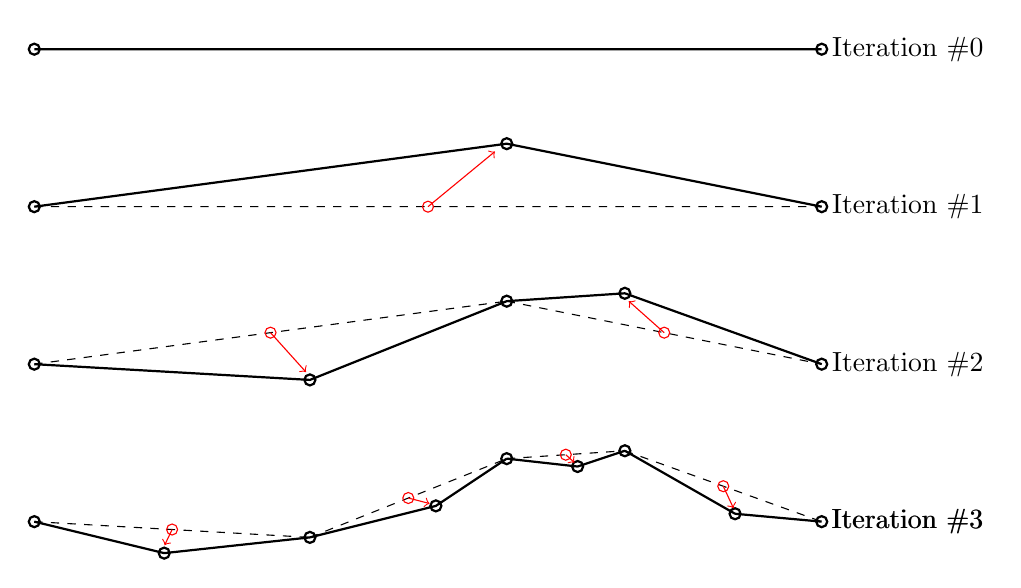
\begin{tikzpicture}
        \draw[thick, black] (0,0) circle(0.07cm) -- (10,0) circle(0.07cm)
        node[anchor=west]{Iteration \#0};
        \draw[dashed, black] (0,-2) circle(0.07cm) -- (10,-2) circle(0.07cm);
        \draw[thick, black] (0,-2) circle(0.07cm) --(6,-1.2) circle(0.07cm) -- (10,-2)
        circle(0.07cm) node[anchor=west]{Iteration \#1};
        \draw[red] (5,-2) circle(0.07cm);
        \draw[red, ->] (5,-2) -- (5.85,-1.3);
        \draw[dashed, black] (0,-4) circle(0.07cm) --(6,-3.2) circle(0.07cm) -- (10,-4) circle(0.07cm);
        \draw[red, ->] (3,-3.6) -- (3.45,-4.1);
        \draw[red, ->] (8,-3.6) -- (7.55,-3.2);
        \draw[red] (3,-3.6) circle(0.07cm);
        \draw[red] (8,-3.6) circle(0.07cm);
        \draw[thick, black] (0,-4) circle(0.07cm) -- (3.5,-4.2) circle(0.07cm) -- (6,-3.2)
        circle(0.07cm) -- (7.5,-3.1) circle(0.07cm) -- (10,-4) circle(0.07cm) node[anchor=west]{Iteration \#2};
        \draw[dashed, black] (0,-6) circle(0.07cm) -- (3.5,-6.2) circle(0.07cm) -- (6,-5.2)
        circle(0.07cm) -- (7.5,-5.1) circle(0.07cm) -- (10,-6) circle(0.07cm) node[anchor=west]{Iteration \#3};
        \draw[thick, black] (0,-6) circle(0.07cm) -- (1.65,-6.4) circle(0.07cm) --
        (3.5,-6.2) circle(0.07cm) -- (5.1,-5.8) circle(0.07cm) -- (6,-5.2)
        circle(0.07cm) -- (6.9,-5.3) circle(0.07cm) -- (7.5,-5.1) circle(0.07cm) --
        (8.9,-5.9) circle(0.07cm) -- (10,-6) circle(0.07cm) node[anchor=west]{Iteration \#3};
        \draw[red] (1.75,-6.1) circle(0.07cm);
        \draw[red] (4.75,-5.7) circle(0.07cm);
        \draw[red] (6.75,-5.15) circle(0.07cm);
        \draw[red] (8.75,-5.55) circle(0.07cm);
        \draw[red, ->] (1.75,-6.1) -- (1.655,-6.3);
        \draw[red, ->] (4.75,-5.7) -- (5.02,-5.77);
        \draw[red, ->] (6.75,-5.15) -- (6.86,-5.25);
        \draw[red, ->] (8.75,-5.55) -- (8.88,-5.83);
    \end{tikzpicture}
\end{center}



\begin{problem}
    Compare the number of iterations necessary for convergence to within $10^{-8}$ for
    both the bisection method and the regula falsi method on several test problems. Find
    example problems where bisection converges faster and examples where regula falsi
    converges faster. Write a test script that clearly indicates to the user which
    equation was being solved, which endpoints were used, and which root finding technique
    performed faster.
\end{problem}


\begin{problem}[Modified from \cite{Chartier}]
    An artillery officer wishes to fire his cannon on an enemy brigade.  He wants to know
    the angle to aim the cannon in order to strike the target.  Follow the steps below to
    arrive at an approximate answer.
    \begin{enumerate}
        \item[(a)] Solve the simple differential equation $v_y'(t) = -g$ by hand where $v_y(t)$
            is the vertical velocity of the canon and gravity is given as $g \approx
            9.8$m/s$^2$.  We don't know the initial velocity so just use $v(0) = v_0$ and
            hence $v_y(0) = v_0 \sin(\theta)$. Note: your answer will have a ``$v_0$'' and a
            ``$\sin(\theta)$'' in it.
        \item[(b)] Solve the differential equation $s_y'(t) = v_y(t)$ by hand for the position
            function $s_y(t)$.  Assume that $s_y(0) = 0$.  Your answer will still have a ``$v_0$'' and a
            ``$\sin(\theta)$'' in it.
        \item[(c)] Solve $s_y(t) = 0$ by hand for $t$ in terms of $v_0$ and $\theta$ to
            find a function for the amount of time the projectile takes to reach the
            ground.
        \item[(d)] In the absence of air resistance the projectile will have a constant
            velocity in the horizontal direction.  Solve the differential equation
            $s_x'(t) = v_0 \cos(\theta)$ for the horizontal position function $s_x(t)$.  
        \item[(e)] The range function $R(v_0,\theta)$ can be found by substituting the
            time from part (c) into the horizontal position function in part (d).  Find
            the function $R(v_0,\theta)$.
        \item[(f)] For a certain projectile and canon the initial velocity is $v_0 =
            126$m/s.  We want to give the artillery officer a distance, $d$, and have them
            calculate the angle to hit the target.  Write MATLAB code to approximate
            $\theta$ in the equation 
            \[ R(126,\theta) = d. \]
            (Hint: remember that we can rewrite the equation $R(126,\theta)=d$ in the form
            $f(\theta) = 0$ for some function $f$ so that we can actually use our
            numerical root finding techniques. See the discussion at the very beginning of
            this chapter.)

            Report a table of values of the form shown below and provide an appropriate
            plot showing your results.  Clearly some distances will be out of range so be
            sure to clearly indicate the range of the weapon.
            \begin{center}
                \begin{tabular}{|c|c|}
                    \hline
                    Distance ($d$ meters) & Angle ($\theta$) \\ \hline \hline
                    0 & \\
                    25 & \\
                    50 & \\
                    100 & \\
                    $\vdots$ & \\ \hline
                \end{tabular}
            \end{center}
    \end{enumerate}
\end{problem}
\hint{
    Remember that solving the equation $R(126,\theta) = d$ is the same as solving the
    equation $R(126,\theta)-d = 0$.  This is the setup you need for all of our root
    finding techniques.
}


\begin{problem}
    Consider our three primary root finding methods: Bisection, Newton's method, and the
    Secant method.  
    \begin{enumerate}
        \item[(a)] For each method give a mathematical situation where you might want to
            use the method and give a mathematical situation where you might not want to
            use the method.  
        \item[(b)] For each of these methods give one example where the method will fail.  
        \end{enumerate}
        Support your arguments with proper mathematics.  You are welcome to argue
        graphically but be sure to fully explain your graphical reasoning.
\end{problem}


\begin{problem}
    Write MATLAB code that produces a loglog plot that compares the convergence rates for
    the bisection method, the regula-falsi method, Newton's method, the secant method, and
    Steffensen's method on a problem where we know the exact answer. See problem
    \ref{prob:newton_convergence} to get you started.
\end{problem}




\begin{problem}
    A {\it fixed point} of a function $f(x)$ is a point that solves the equation $f(x) =
    x$.  Fixed points are interesting in iterative processes since fixed points don't
    change under repeated application of the function $f$.  

    For example, consider the function $f(x) = x^2 - 6$.  The fixed points of $f(x)$ can be found by
    solving the equation $x^2 - 6 = x$ which, when simplified algebraically, is $x^2 - x -
    6 = 0$.  Factoring the left-hand side gives $(x-3)(x+2)=0$ which implies that $x=3$
    and $x=-2$ are fixed points for this function. That is, $f(3) = 3$ and $f(-2) = -2$.
    Notice, however, that finding fixed points is identical to a root finding problem.
    \begin{enumerate}
        \item[(a)] Use a numerical root-finding algorithm to find the fixed points of the
            function $f(x) = x^2 - 6$ on the interval $[0,\infty)$.
            \item[(b)] Find the fixed points of the function $f(x) =
                \sqrt{\frac{8}{x+6}}$.
    \end{enumerate}
\end{problem}

\begin{problem}
    In Single Variable Calculus you studied methods for finding local and global extrema
    of functions. You likely recall that part of the process is to set the first
    derivative to zero and to solve for the independent variable (remind yourself why
    you're doing this).  The trouble with this process is that it may be very very
    challenging to do the algebraic solve by hand.  This is a perfect place for Newton's
    method or any other root finding techinque! \\
    Find the local extrema for the function $f(x) = x^3(x-3)(x-6)^4$ and explicitly
    demonstrate, without the use of a plot, that you have found all of the local extrema.
\end{problem}
\hint{
    Recall that if the derivative of a single variable function is zero then the function
    has a possible local extrema.  In this problem it is likely best to find the first and
    second derivatives on paper before writing any code.
}


\begin{problem}\label{prob:mv_newton}
    The Newton's method that we derived in this chapter is only applicable to functions
    $f: \mathbb{R} \to \mathbb{R}$ (functions mapping a real number to a real number).
    What about vector-valued functions?  In particular, we would like to have an analogous
    method for finding roots of a function $F$ where $F: \mathbb{R}^n \to \mathbb{R}^n$.

    Let $\bx$ be a vector in $\mathbb{R}^n$, let 
    \[ F(\bx) = \begin{pmatrix} f_1(\bx) \\ f_2(\bx) \\ \vdots \\ f_n(\bx) \end{pmatrix} \]
    be a vector valued function, and let $J$ be the Jacobian matrix
    \[ J(\bx) = 
        \begin{pmatrix} \partial f_1 / \partial x_1(\bx) & \partial f_1 / \partial
            x_2(\bx) & \cdots
            & \partial f_1 / \partial x_n(\bx) \\ 
         \partial f_2 / \partial x_1(\bx) & \partial f_2 / \partial x_2(\bx) & \cdots &
         \partial f_2 / \partial x_n(\bx) \\ 
         \vdots & \vdots & \ddots & \vdots \\
         \partial f_n / \partial x_1(\bx) & \partial f_n / \partial x_2(\bx) & \cdots & \partial f_n /
     \partial x_n(\bx) \end{pmatrix} \]
    By analogy, the multi-dimensional Newton's method is
    \[ \bx_{n+1} = \bx_n -  J^{-1}(\bx_n)F(\bx_n) \]
    where $J^{-1}(\bx_n)$ is the inverse of the Jacobian matrix evaluated at the point
    $\bx_n$.
    \begin{enumerate}
        \item[(a)] Write MATLAB code that accepts any number of functions and an initial
            vector guess and returns an approximation to the root for the problem $F(\bx) = \bo$.
        \item[(b)] Test your code on the system of nonlinear equations
            \begin{flalign*}
                1+x^2 - y^2 + e^x\cos(y) &= 0 \\
                2xy + e^x\sin(y) &=0.
            \end{flalign*}
            Note here that $f_1(x,y) = 1+x^2 - y^2 + e^x\cos(y)$ and $f_2(x,y) = 2xy + e^x
            \sin(y)$.
        \item[(c)] Use Newton's method to find an approximate solution to the system of
            equations
            \begin{flalign*}
                x^2 + y^2 + z^2 &= 100 \\
                xyz &= 1 \\
                x - y - \sin(z) &= 0
            \end{flalign*}
    \end{enumerate}
\end{problem}
\hint{
    If you want to evaluate the matrix-vector multiplication $J^{-1}(\bx_n) F(\bx_n)$ then
    you are really looking for the solution $\bu$ to the system of equations $J(\bx_n) \bu =
    F(\bx_n)$ and you can use MATLAB's backslash command to get it quickly. 

    For part (c) be sure to first make the right-hand side zero.
}



